\documentclass[tikz,border=8pt]{standalone}
\usepackage[T1]{fontenc}\usepackage{lmodern}\usepackage{pgfplots}\pgfplotsset{compat=1.18}
\begin{document}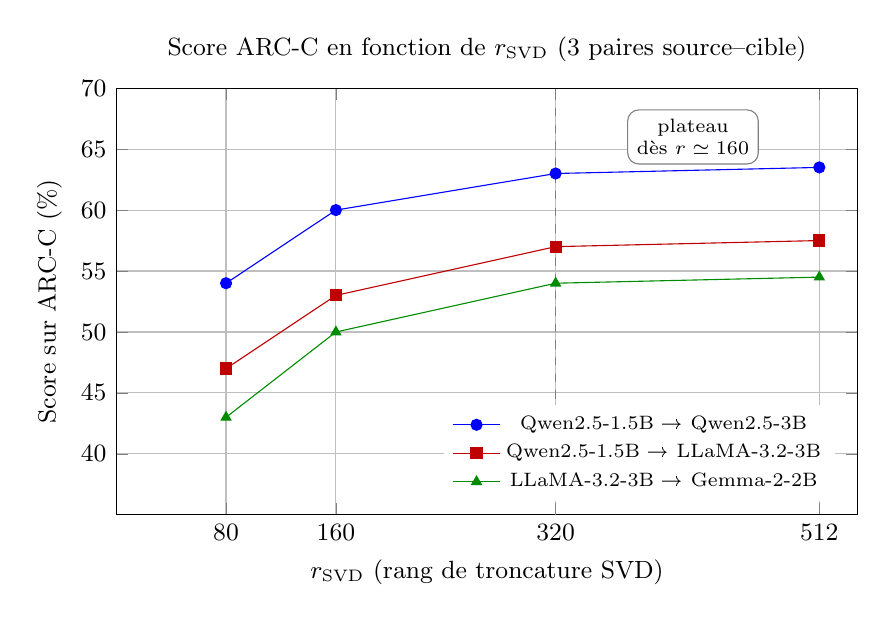
\begin{tikzpicture}
\begin{axis}[width=11cm,height=7cm,font=\small,title={Score ARC-C en fonction de $r_{\mathrm{SVD}}$ (3 paires source–cible)},xlabel={$r_{\mathrm{SVD}}$ (rang de troncature SVD)},ylabel={Score sur ARC-C (\%)},xmin=0,xmax=540,ymin=35,ymax=70,xtick={80,160,320,512},ytick={40,45,50,55,60,65,70},grid=major,legend pos=south east,legend style={font=\scriptsize,fill=white,draw=none}]
% Schematic digitization: original source image does not expose a numerical table.
\addplot[blue,mark=*] coordinates {(80,54)(160,60)(320,63)(512,63.5)};\addlegendentry{Qwen2.5-1.5B → Qwen2.5-3B}
\addplot[red!75!black,mark=square*] coordinates {(80,47)(160,53)(320,57)(512,57.5)};\addlegendentry{Qwen2.5-1.5B → LLaMA-3.2-3B}
\addplot[green!55!black,mark=triangle*] coordinates {(80,43)(160,50)(320,54)(512,54.5)};\addlegendentry{LLaMA-3.2-3B → Gemma-2-2B}
\draw[dashed,gray] (axis cs:320,35)--(axis cs:320,70);\node[anchor=south west,font=\scriptsize] at (axis cs:324,37) {choix papier : $r_{\mathrm{SVD}}=320$};
\node[draw=gray,fill=white,rounded corners,font=\scriptsize,align=center] at (axis cs:420,66) {plateau\\dès $r\simeq160$};
\end{axis}\end{tikzpicture}\end{document}
